Consider the following order-dependent function, $F_l(\zeta)$, given by
\begin{equation}\label{eq:02_Acoustical_Theory:Fl_zeta}
F_l(\zeta) = \zeta l h_l (\zeta l).
\end{equation}
This family of functions is plotted in \figref{fig:02_Acoustical_Theory:Nearfield_Amplification}.
From this figure, we note that amplification occurs below $\zeta = 1$, with the slope of the amplification increasing with increasing $l$.

% Near-field amplification
\begin{figure}[t]
\centering
  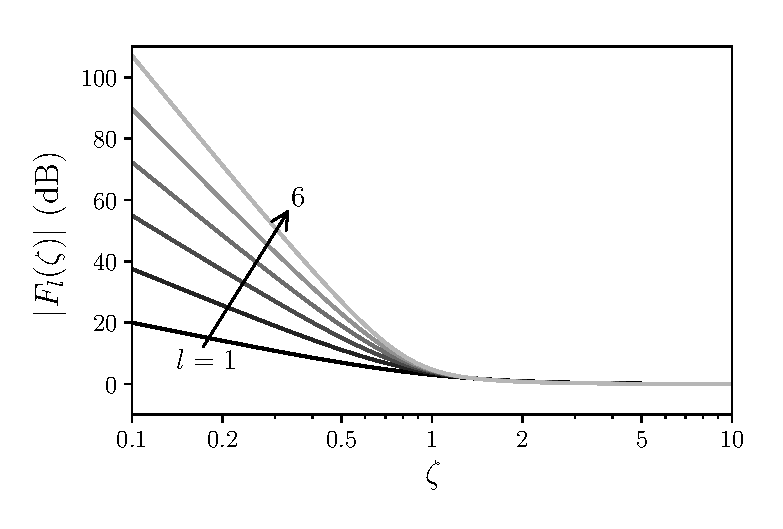
\includegraphics[width = 0.6\textwidth]{02_acoustical_theory/figures/nearfield_amplification.eps}
  \caption[Magnitudes of the family of functions given in \eqnref{eq:02_Acoustical_Theory:Fl_zeta}.]{
  Magnitudes of the family of functions given in \eqnref{eq:02_Acoustical_Theory:Fl_zeta} for increasing values of $l$ from $l = 1$ (black curve) to $6$ (lightest gray).
  If the nondimensional wavenumber $k s_0 / l$ is substituted for $\zeta$, then these curves illustrate the near-field amplification introduced when encoding a point-source into ambisonics (see \eqnref{eq:02_Acoustical_Theory:Nearfield_Amplification} and cf.~\citet[Fig.~4]{Daniel2003b}).}
  \label{fig:02_Acoustical_Theory:Nearfield_Amplification}
\end{figure}

If we let $\zeta = k s_0 / l$, we can relate this function to the distance-coding term of the point-source encoding filters (as given in \eqnref{eq:02_Acoustical_Theory:PointSource_An}) by
\begin{equation}\label{eq:02_Acoustical_Theory:Nearfield_Amplification}
\left| s_0 \frac{A_n (k)}{Y_n (\hat{s}_0)} \right| = \left| k s_0 h_l (k s_0) \right| = \left| F_l \left( \frac{k s_0}{l} \right) \right|,
\end{equation}
where $|\cdot|$ denotes the absolute value (or modulus or magnitude) of the argument.
From this relationship, we see that increasing (or decreasing) the source distance $s_0$ has two effects on the resulting ambisonics signals:
\begin{enumerate}
\item the overall amplitude of each ambisonics signal decreases (increases), and
\item the frequency below which the amplification occurs decreases (increases).
\end{enumerate}
In particular, the ambisonics signals are amplified at frequencies below $k = l / s_0$ (cf.~\citep[section 2.1]{Daniel2003b}).

To prevent excessive low-frequency amplification from this effect, we define for all ambisonics orders $l \in [1, L_\textrm{in}]$, an order-dependent, zero-phase high-pass Butterworth filter, the frequency response of which is given by
\begin{equation}\label{eq:02_Acoustical_Theory:NearField_HPF}
H_l(f) = 1 - \frac{1}{\sqrt{1 + \left( \frac{f}{f_l} \right)^l}},
\end{equation}
where $f_l$ is the corner frequency of the $l^\textrm{th}$ filter,
which, unless stated otherwise, we choose to be $f_l = (200 \times l)$~Hz.

As shown above, the frequency at which the near-field amplification occurs increases as the distance between the source and microphone decreases.
However, the compensation filters given in~\eqnref{eq:02_Acoustical_Theory:NearField_HPF} are independent of source position, which will lead to excessive low-frequency amplification (due to insufficient compensation) at small source distances and excessive low-frequency attenuation at large source distances.
The plots in \figref{fig:02_Acoustical_Theory:Nearfield_Compensation} illustrate this effect for $s_0 = 0.05, 1$~m.
This approach, while inexact, is representative of practical reality since, in general, the source position(s) may be unknown.
Indeed, the Eigenmike by mh acoustics uses distance-independent compensation filters \citep[section 4.3]{EigenUnitsManual2018}.
(In the experimental validation presented in \chapref{chap:10_Experimental_Validation}, we use distance-independent compensation filters to match those of the Eigenmike.)

\begin{figure}[t]
    \centering
    \begin{subfigure}[b]{0.49\textwidth}
        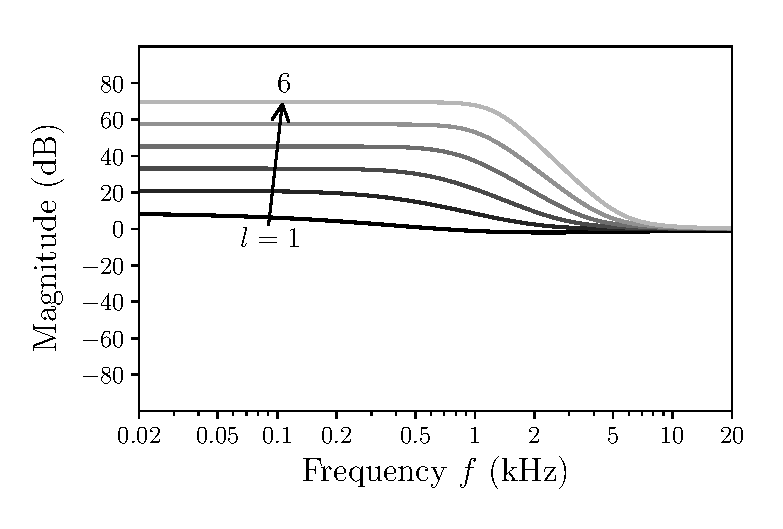
\includegraphics[width=\textwidth]{02_acoustical_theory/figures/nearfield_compensation_5cm.eps}
        \caption{$s_0 = 0.05$~m}
    \end{subfigure}
    \hfill
    \begin{subfigure}[b]{0.49\textwidth}
        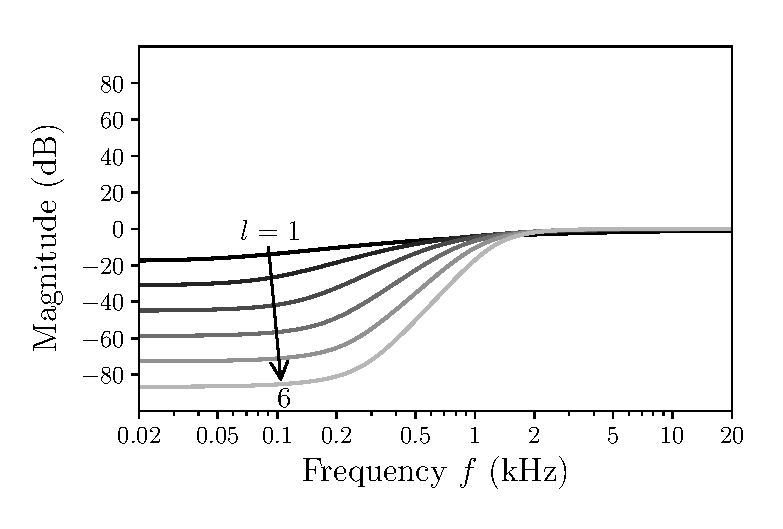
\includegraphics[width=\textwidth]{02_acoustical_theory/figures/nearfield_compensation_100cm.eps}
        \caption{$s_0 = 1$~m}
    \end{subfigure}
\caption[Residual near-field amplification after compensation.]{
Residual near-field amplification for two different source distances after compensation with the Butterworth high-pass filter (see \eqnref{eq:02_Acoustical_Theory:NearField_HPF}).
The magnitude spectra have been multiplied by $s_0$ in order to remove the vertical offset caused by the overall distance attenuation.}
\label{fig:02_Acoustical_Theory:Nearfield_Compensation}
\end{figure} %%NOTE%% vertical axis label is too complicated: |A H| s or something